\section*{Question 4}


\begin{enumerate}[(a)]

\item Here we create the long-short portfolio. The long-short portfolio is created by taking the difference between the returns of the highest and the lowest portfolio. The result is shown in the figure \ref{fig:3c}.
\begin{figure}
    \centering
    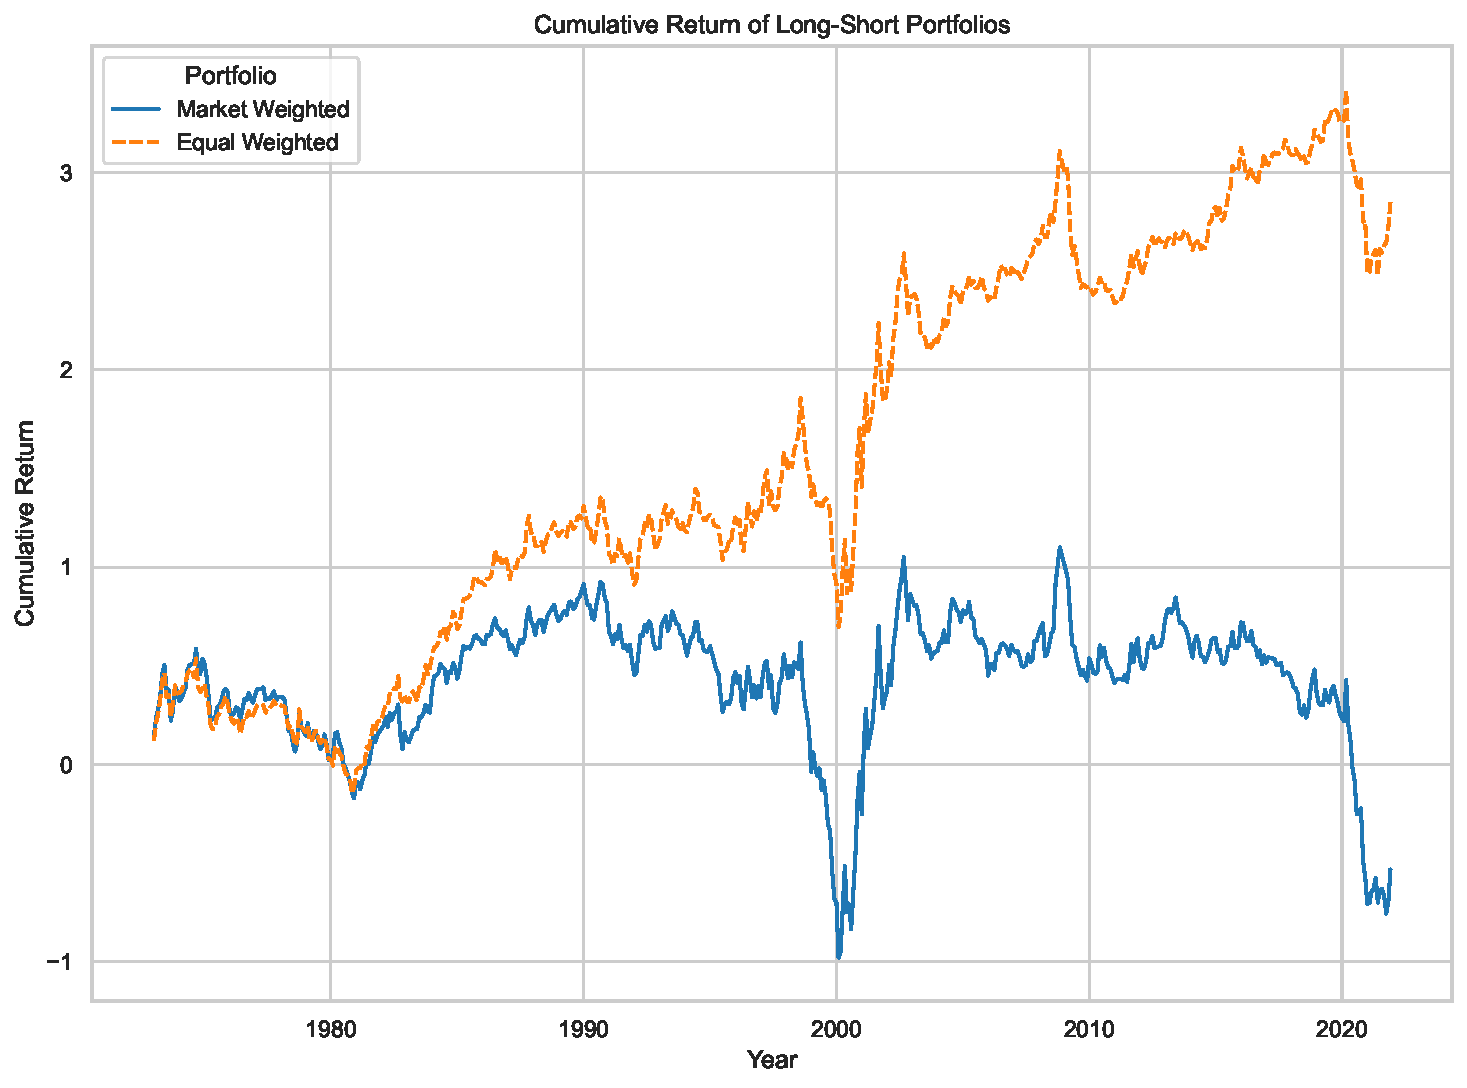
\includegraphics[width=0.6\textwidth]{Out/4_3.pdf}
    \caption{Time series of the average returns of the long-short portfolio.}
    \label{fig:3c}
\end{figure}

Now we can test the CAPM, Fama-French 3 factors and the Fama-French 5 factors, Carhart, and HXZ models. You can find the function that I write to test the null hypothesis that $\alpha_{LS} =0$. I will get the p-value of the test.   



\begin{table}[htbp]
    \caption{$\alpha$ test for long-short portfolio with different models}
    \begin{tabularx}{\linewidth}{CC}
        \caption*{Equal Weighted }
        \begin{tabular}{lcc}
\toprule
 & $\alpha$ & $Pvalue$ \\
\midrule
CAPM & 0.011 & 0.000 \\
FF3 & 0.008 & 0.000 \\
CAR & 0.005 & 0.005 \\
FF5 & 0.004 & 0.025 \\
HXZ & 0.002 & 0.245 \\
\bottomrule
\end{tabular}

        &
        \caption*{Market Weighted }
        \begin{tabular}{lcc}
\toprule
 & $\alpha$ & $Pvalue$ \\
\midrule
CAPM & 0.005 & 0.040 \\
FF3 & 0.003 & 0.170 \\
CAR & 0.000 & 0.825 \\
FF5 & -0.002 & 0.221 \\
HXZ & -0.004 & 0.103 \\
\bottomrule
\end{tabular}

    \end{tabularx}
\end{table}
\item 

\begin{table}[htbp]
    \caption{$\alpha$ test long-short portfolio for in and out of sample with equal weighting}
    \begin{tabularx}{\linewidth}{CC}
        \caption*{Sample period }
        \begin{tabular}{lcc}
\toprule
{} &  \$\textbackslash alpha\$ &  \$Pvalue\$ \\
\midrule
CAPM &     0.011 &     0.000 \\
FF3  &     0.007 &     0.002 \\
CAR  &     0.005 &     0.023 \\
FF5  &     0.004 &     0.107 \\
HXZ  &     0.004 &     0.141 \\
\bottomrule
\end{tabular}

        &
        \caption*{Post-publication period}
        \begin{tabular}{lcc}
\toprule
 & $\alpha$ & $Pvalue$ \\
\midrule
CAPM & 0.014 & 0.000 \\
FF3 & 0.013 & 0.000 \\
CAR & 0.010 & 0.000 \\
FF5 & 0.007 & 0.002 \\
HXZ & 0.004 & 0.077 \\
\bottomrule
\end{tabular}

    \end{tabularx}
\end{table}

\begin{table}[htbp]
    \caption{$\alpha$ test long-short portfolio for in and out of sample with market weighting}
    \begin{tabularx}{\linewidth}{CC}
        \caption*{Sample period }
        \begin{tabular}{lcc}
\toprule
{} &  \$\textbackslash alpha\$ &  \$Pvalue\$ \\
\midrule
CAPM &     0.007 &     0.009 \\
FF3  &     0.003 &     0.112 \\
CAR  &     0.002 &     0.493 \\
FF5  &     0.001 &     0.746 \\
HXZ  &     0.002 &     0.596 \\
\bottomrule
\end{tabular}

        &
        \caption*{Post-publication period}
        \begin{tabular}{lcc}
\toprule
 & $\alpha$ & $Pvalue$ \\
\midrule
CAPM & 0.007 & 0.117 \\
FF3 & 0.006 & 0.058 \\
CAR & 0.004 & 0.207 \\
FF5 & -0.000 & 0.877 \\
HXZ & -0.003 & 0.373 \\
\bottomrule
\end{tabular}

    \end{tabularx}
\end{table}


\end{enumerate}